\documentclass[12pt]{article}
\usepackage[T1]{fontenc}
\usepackage[ngerman]{babel} % german as language
\usepackage{csquotes}
\usepackage[onehalfspacing]{setspace} % 1.5 Zeilenabstand
\usepackage{parskip} % for paragraph line skip
\usepackage{fancyhdr} % for headers
\fancyhf{}
\fancyhead[C]{\nouppercase{\firstmark}}
\renewcommand{\headrulewidth}{0pt} % change line under header
\renewcommand{\footrulewidth}{0pt}
\pagestyle{fancy}
\setlength{\headheight}{15.04742pt}
\fancypagestyle{maintext}{ % pagestyle for main text for page numbers
    \fancyhf{}
    \fancyhead[C]{\nouppercase{\firstmark}}
    \fancyfoot[C]{\thepage}
    \renewcommand{\headrulewidth}{0pt}
    \renewcommand{\footrulewidth}{0pt}
}
% Update \sectionmark to show first section in header
\renewcommand{\sectionmark}[1]{%
    \markboth{\thesection\ #1}{}
}
\renewcommand{\subsectionmark}[1]{}

% for tables/figures
\usepackage{graphicx}
\usepackage{caption}
\usepackage{array}
\graphicspath{ {figures/} } % set path to figures
\renewcommand{\listfigurename}{Abbildungsverzeichnis}
\renewcommand{\listtablename}{Tabellenverzeichnis}

% Appendix
\usepackage[toc,page]{appendix}
\renewcommand\appendixname{Anhang} % Change name to German
\renewcommand\appendixpagename{Anhang}
\renewcommand\appendixtocname{Anhang}


% \usepackage{sectsty} -> falls section font size 14 haben muss
% \sectionfont{\large\bfseries}

% use geometry for page layout
\usepackage[a4paper, left=2.5cm, right=2.5cm, top=2.5cm, bottom=2cm]{geometry}

% Citation: BibLaTeX als author-year style, benötigt xelatex->biber->xelatex(2x) als recipe!
\usepackage[
backend=biber,
style=authoryear]{biblatex}
\addbibresource{refs.bib}

% Start des Dokuments
\begin{document}

% Add centered Title page
\begin{titlepage}
    \begin{center}
        \vspace*{0.5cm}
            
        \LARGE
        \textbf{Erstellung einer Unterrichtsreihe mit dem Fokus auf eine heterogene Gruppe}
            
        \vspace{0.2cm}
        \Large
        Variante B\\
        Methodenschwerpunkt
            
        \vspace{2cm}
            
        \textbf{Lukas Schaffrath}\\
        Matrikelnummer: 411793\\
        Lehramt Technik/Englisch\\
        Master für Gymnasien und Gesamtschulen
            
        \vspace{2cm}
            
        Seminar: Umgang mit Heterogenität im Technikunterricht\\
        Dozent: Gerrit Albert
            
        \vspace{2cm}
            
            
        \Large
        I. Physikalisches Institut IA\\
        RWTH Aachen University\\
        Sommersemester 2024\\
        02. September 2024
            
    \end{center}
\end{titlepage}

% Add table of contents with emtpy page number
\addtocontents{toc}{\protect\thispagestyle{empty}}
\tableofcontents

% List of figures and tables
\newpage
\thispagestyle{empty}
\listoffigures
\vspace{0.5cm}
\listoftables


% New page, page count to 1
\newpage
\setcounter{page}{1}
\pagestyle{maintext}

% Add Main Text
\section{Einleitung}
In dieser Hausarbeit wird eine beispielhafte Unterrichtsreihe entworfen, die im gymnasialen oder gesamtschulischen Technikunterricht eingesetzt werden kann. Fokussiert wird die Methodik bezogen auf die Herausforderungen der inklusiven Bildung, denen sich Lehrer*innen im Alltag annehmen müssen. Ziel ist es eine möglichst inklusive Unterrichtsreihe anhand einer Beispiel-Lerngruppe und zwei Beispiel-Unterrichtsstunden zu entwickeln, vorzustellen und zu bewerten. Sie ist darauf ausgerichtet, inklusives Lernen zu fördern und individuelle Lernangebote für Schülerinnen und Schüler mit Förderbedarf so zu integrieren, dass inklusives Lernen bestmöglich ermöglicht wird. Technikunterricht bietet durch die handlungsorientierte Natur eine Möglichkeit, praxisorientierte Fähigkeiten zu fördern, aber auch technische Grundkenntnisse zu vermitteln. Handwerkliche Projekte, wie der Bau eines Vogelhauses wie er hier vorgestellt wird, fördern nicht nur motorische Fähigkeiten, sondern auch Problemlösungs- und Planungskompetenzen, während sie Möglichkeiten bieten, heterogene Gruppen zu vereinen und Schülerinnen und Schüler mit Förderbedarf einzubinden.

Heterogenität stellt einen zentralen Aspekt der modernen Schulbildung und eine wesentliche Herausforderung für Lehrkräfte dar, da Schülerinnen und Schüler unterschiedlichste Lernvoraussetzungen, Fähigkeiten und Förderbedarfe mitbringen. Durch die zunehmende Bedeutung der individuellen Schüler-Förderung, um Chancengleichheiten und Bildungserfolge für Jedermann zu gewährleisten, ist der Umgang mit Heterogenität für Lehrer*innen unumgänglich. Ein Einblick in Heterogenität und inklusives Lernen wird in Kapitel zwei gegeben, inklusive der Vorstellung zweier Förderschwerpunkte, die in der Planung der Unterrichtsreihe berücksichtigt werden. Daraufhin wird der theoretische Hintergrund der Unterrichtsreihe beleuchtet, was die Vorstellung der imaginären Lerngruppe, die Begründung des Themas, die Lernziele und den Verlauf der Unterrichtsreihe beinhaltet. Zuletzt werden zwei Unterrichtsstunden beispielhaft vorgestellt, um einen detaillierten Einblick in den inklusiven Unterrichtsablauf zu bieten. Das Lernmaterial wird dabei erläutert und ist im Anhang der Arbeit auffindbar.


\section{Grundlagen}
Im Folgenden werden die Grundlagen, auf denen die theoretische Ausarbeitung der Unterrichtsreihe beruht, vorgestellt, um ein bestmögliches Verständnis für die Auswahl der didaktischen Praktiken zu ermöglichen. Für die gestaltung einer Unterrichtsreihe, die besonders inklusives Lernen innerhalb einer heterogenen Schüler-Gruppe, muss der Begriff der Heterogenität und des inklusiven Lernens definiert werden, was im ersten Unterkapitel versucht wird. Des Weiteren werden die zwei Förderschwerpunkte, die in der vorgestellten Lerngruppe vorkommen, spezifiziert und Hinweise auf den Umgang mit diesen gewährleistet.

\subsection{Heterogenität und inklusives Lernen}
Da jede Gruppe von Schülerinnen und Schüler zu einem bestimmten Grad \textit{heterogen} ist, ist der Umgang mit jener für Lehrer*innen von höchster Bedeutung, um einen effektiven Unterricht zu gestalten. Heterogenität bezeichnet \enquote{sowohl soziale oder kulturelle
Unterschiede als auch die divergenten leistungsbezogenen
Ausgangsbedingungen der Schülerschaft} \autocite[87]{grohlich_wirkt_2009}, und ist nach dieser Definition in jeder Schüler-Gruppe auffindbar. Sie umfasst verschiedene Dimensionen, wie z.B. die Vorerfahrungen, die soziale Herkunft, das Geschlecht, das Alter, die Bildungsorientierung oder die Motivation \autocite[vgl.][]{trautmann_heterogenitat_2011}. Um dieser vorhandenen heterogenen Gruppe, und jedem einzelnen Schüler darin (besonders Kindern, mit besonderen Förderbedarfen) didaktisch gerecht zu werden, ist ein inklusives Lern- und Lehrkonzept von höchster Bedeutung.

Daher wurde die hier dargestellte Unterrichtsreihe an den vier Kardinalsmerkmalen der Inklusion nach Hans Wocken orientiert: (1) inklusiver Personenkreis, (2) inklusives Curriculum, (3) inklusiver Unterricht und (4) inklusive Professionalität. Der erste Punkt meint, dass Kinder nicht als \textit{anders} aufgenommen und behandelt werden, da in einem inklusiven Schulsystem keine \textit{anderen} Kinder existieren. Jeder Schüler wird, egal wie sich die heterogene Gruppe zusammensetzt, als individuell förderbare Person angesehen, und dahingehend gefördert. Dies ist was im zweiten Punkt impliziert wird: es gibt ein individuelles Curriculum, das jedem Kind individuell gerecht wird, und alle Kinder einschließt. Die dritte Dimension beinhaltet, dass gemeinsame Lernsituationen hervorgerufen werden, um so den Kindern das inklusive Lernsystem anzueignen. Die vierte Dimension ist auf die Lehrer*innen bezogen, und meint, dass ein multiprofessionelles Team von Lehrer*innen den Unterricht gestaltet und unterstützt \autocite[vgl.][S.4f.]{wocken_inklusive_2019}. Nur unter berücksichtigung dieser vier Kardinalsmerkmale kann jedes Kind individuell und bestmöglich gefördert werden, und ein inklusives Schulsystem existieren.

\subsection{Förderschwerpunkt \textit{Hören und Kommunikation}}
In der vorgstellten Unterrichtsreihe wird der Förderschwerpunkt \textit{Hören und Kommunikation} fokussiert, da ein Schüler der heterogenen Lerngruppe diesem zugehört (siehe 3.1). Dieser Förderschwerpunkt \enquote{umfasst Schülerinnen und Schüler mit unterschiedlichen Arten und Graden von peripheren und zentralen Hörstörungen.} \autocite[vgl.][]{prof_dr_thomas_kaul_forderschwerpunkt_2016}. Darunter fallen u.a. verschiedene Arten der Schwerhörigkeit, aber auch einseitige Hörschädigungen, sowie Ertaubung. Auch wenn die meisten Schülerinnen und Schüler, die diesem Förderschwerpunkt angehören, Hörhilfen tragen, wird die Hörschädigung oft nicht vollständig durch diese ausgeglichen, und die Schüler könnten weitere Förderbedarfe mitbringen. Des Weiteren sind Schülerinnen und Schüler mit diesem Förderbedarf oft unauffällig und ihre Situation wird falsch eingeschätzt. Deshalb sollten Lehrer*innen im inklusiven Schulsystem Vorbereitungen treffen, um die Schüler mit diesem Förderbedarf ausreichend zu fördern. Dazu zählt das Einhalten organisatorischer Rahmenbedingungen, darunter optische (ein ausgeleuchtetes Klassenzimmer, Blickkontakt zur Lehrer*in gewährleisten, einen geringen Abstand zwischen den Schülern und Sprechern herstellen), akustische (z.B. Geräusch und Lärmquellen vermeiden) und das Klassenklima (Aufklärung der Mitschüler, Sonderrollen für Schüler mit Hörschädigung vermeiden). Ebenso wichtig ist die Sicherung der sprachlichen und kommunikativen Barrierefreiheit, bezogen auf die Sprache der Lehrer*innen, aber auch in Unterrichtsgesprächen. Hier helfen Gesprächsregeln im Unterricht (z.B. kein Durcheinanderreden zu dulden) und Maßnahmen der Verschriftlichung, damit Schülerinnen und Schüler mit einer Hörschädigung nicht benachteiligt werden. Eine klare Unterrichtsstruktur und Visualisierungen sollten Bestandteil des Unterrichts sein, genauso wie  eine Verstehenssicherung, um klarzustellen, dass die benachteiligten Schülerinnen und Schüler den Unterrichtsinhalten folgen kann. \autocite[vgl.][]{prof_dr_thomas_kaul_forderschwerpunkt_2016}.

\subsection{Förderschwerpunkt \textit{Lernen}}
Ebenso wie der zuvor vorgestellte Förderschwerpunkt \textit{Hören und Kommunikation} wird hier der Förderschwerpunkt \textit{Lernen} vorgestellt, um die in der Unterrichtsreihe vorgestellten didaktischen Motive, bezogen auf die beiden Schüler mit Förderbedarf die der Lerngruppe angehören (siehe 3.1), nachvollziehen zu können. Unter diesem Förderschwerpunkt versteht man \enquote{Lern- und Entwicklungsstörungen}, welche \enquote{erhebliche Beeinträchtigungen im Lernen, der Sprache sowie
in der emotionalen und sozialen Entwicklung} hervorrufen und sich häufig gegenseitig oder wechselseitig Verstärken und Beeinflussen \autocite{qua-lis_nrw_kurz-informationen_2018}. Auch wird eine hohe Diskrepanz zwischen dem inhaltlich Vorausgesetzten und den aktuellen Leistungen des Schüler vorausgesetzt. Hierunter fallen unter anderem ADHS, Lese-Rechtschreib-Schwäche oder Diskalkulie und geht oft mit verschiedenen Erscheinungsformen einher, wie zum Beispiel erschwerte Lebenssituationen, Entwicklungsverzögerungen, Ängsten, einer begrenzten Konzentrations- und Aufmerksamkeitsspanne, hohe Ablenkungsbereitschaft und Vermeidungsverhalten. Im schulischen, inklusiven Unterricht helfen kooperative, offene Unterrichtsformen, die Aufbereitung von Lerngegenständen, eine emotionale Anbindung an Themen, eine schrittweise Inhaltsvermittlung, handlungsorientierte Lernangebote, sowie feste Strukturen und klare Instruktionen, um die Schülerinnen und Schüler bestmöglich zu fördern \autocite[vgl.][]{qua-lis_nrw_kurz-informationen_2018}.

\section{Vorstellung der Unterrichtsreihe}
\subsection{Die Lerngruppe}
Die zur Vorbereitung der Unterrichtsreihe genutzte, beispielhafte Lerngruppe besteht aus 28 Schülerinnen und Schüler der Klasse 5 einer Gesamtschule. Darunter befinden sich 19 weibliche und 9 männliche Schülerinnen und Schüler, wozu zwei Schüler mit Förderbedarf zählen. Wie in den vorherigen Kapiteln angedeutet, zählt zu diesen ein männlicher Schüler, Jens, der eine Hörschädigung hat und somit dem Förderschwerpunkt \textit{Hören und Kommunikation} angehört. Desweiteren befindet sich eine weibliche Schülerin namens Jana in der Lerngruppe, die augrund von Legasthenie dem Förderschwerpunkt \textit{Lernen} angehört. 

\subsection{Vorkenntnisse}
Die Lerngruppe ist aufgrund des Fakts, das sich die Schülerinnen und Schüler in der ersten Klassenstufe der Gesamtschule befinden und erst vor kurzem als Gruppe zusammengekommen sind, sehr heterogen, weshalb die Schülerinnen und Schüler verschiedene Vorkenntnisse und Erfahrungen mitbringen, die sich auf unterschiedliche Bereiche des Technikunterrichts erstrecken. Einige Schüler haben bereits in der Grudschule im Fach Werken grundlegende handwerkliche Fähigkeiten erworben und Erfahrungen im Umgang mit einfachen Werkzeugen wie Sägen, Hämmern und Schraubendrehern gesammelt. Zudem verfügen einige über Kenntnisse in der Materialkunde, die sie durch den Werkunterricht erworben haben. Durch verschiedene Gruppenprojekte in der Grundschule sind die Schüler mit Teamarbeit vertraut und haben gelernt, gemeinsam an Aufgaben zu arbeiten. Grundlegende Sicherheitsregeln für den Umgang mit Werkzeugen und Materialien sind den Schülerinnen und Schülern ebenfalls bekannt. Darüber hinaus haben die Schülerinnen und Schüler Erfahrungen in der kreativen Gestaltung von Projekten gesammelt, dies nicht nur im Technikunterricht, sondern beipielsweise im Kunstunterricht. Diese Vorkenntnisse bilden eine solide Grundlage für die geplante Unterrichtsreihe im Technikunterricht, da Sie auf ihre bisherigen Erfahrungen zurückgreifen und diese im Rahmen des neuen Projekts vertiefen und erweitern können.

\subsection{Themenfindung}
Das Thema der Unterrichtsreihe ist der \textit{Bau eines einfachen Vogelhauses aus Holz}, welches gewählt wurde, weil der Bau relativ einfach gestaltet werden kann, und die benötigten Werkzeuge und Materialien in vielen Schulen vorhanden sein könnten, und das Zusatzmaterial günstig besorgbar ist. Dazu zählen Bauwerkzeuge und -materialien, wie die selbsterstellten Baupläne (siehe Anhänge), Papier und Stifte, dünne 3mm dicke Sperrholzplatten, Holzleim, Japansägen und Maßbänder, Schleifpapier, Pinsel und Farben zur Personalisierung, sowie Sicherheitsausrüstung, wozu Schutzbrillen und Handschuhe zählen. Des Weiteren wurde dieses Thema gewählt, da die Aufgaben motorischer und handlungsorientierter Natur sind, mit verschiedenen didaktischen Überlegungen erstellt werden können, und z.B. durch Verschönerungen, Bohrungen oder weitere äußere Bauten erweitert werden können, um diese an die schnellerarbeitenden Schülerinnen und Schüler anzupassen.

Bezogen auf den Kernlehrplan NRW für Gymnasien und Gesamtschulen im Fach Technik, wird hier das Inhaltsfeld 2 \enquote{Planung und Herstellung technischer Systeme} \Autocite[][S. 13]{ministerium_fur_schule_und_bildung_kernlehrplan_2020} fokussiert und verschiedene Kompetenzbereiche abgedeckt. Dazu zählt die Sachkompetenz, welche durch die begrifflichen Unterscheidungen des Materials und der Werkzeuge inkludiert wird, die Methodenkompetenz durch die Erschließung und den Bau eines technischen Systems, sowie die Urteilskompetenz aufgrund der begründeten, eigenen Planung und des Baus, als auch die Handlungskompetenz durch das Lernen mit dem Umgang des Werkzeugs und Materials \Autocite[vgl.][S. 12]{ministerium_fur_schule_und_bildung_kernlehrplan_2020}. 

\subsection{Umsetzung der Unterrichtsreihe}
\subsubsection{Lernziele}
Die hier erstellten Lehr- und Lernziele richten sich nach der Kategorisierung, wie sie von Bloom aufgeführt wurden \autocite[vgl.][]{sachsisches_e-competence_zertifikat_formulierung_2010}. Als kognitives Lernziel für die Unterrichtsreihe wurde "Die Schülerinnen und Schüler geben den grundlegenden Aufbau eines Vogelhauses wieder und benennen einzelne Bauteile und deren Zusammenhang" formuliert. Das affektive Lehrziel lautet "Die Schülerinnen und Schüler beachten die erlernten Sicherheitsregeln im Umgang mit Werzeugen", was auf die Bildung angemessener Werturteile abzielt. Das psychomotorische Lehrziel umfasst "Die Schülerinnen und Schüler wenden das gelernte an und erproben dies beim Bau eines realen Bauwerks", was die Beherrschung von Bewegungsabläufen und Verhaltensweisen (in Form von handwerklichen Fähigkeiten) beinhaltet. Alle Lernziele entsprechen den Formulierungshilfen von Sandra Döhring und der von ihr formulierten Klassifizierung, um die Wiedergabe von Fakten, das Verstehen von komplexen Zusammenhängen und das Anwenden von erworbenem Wissen in neuen Situationen zu inkludieren \autocite[vgl.][]{sachsisches_e-competence_zertifikat_formulierung_2010}.

\subsubsection{Verlauf}
Im Folgenden wird der Unterrichtsverlauf dargestellt, so wie er in der untenstehenden Tabelle geplant wurde (siehe Tabelle 1). Die Unterrichtsreihe umfasst vier Unterrichtsstunden, inklusive einer Einführungsstunde und drei Arbeitsstunden, wobei die vierte und letzte Stunde den Abschluss in Form einer kreativen Auslass- und Pufferstunde für die Fertigstellung des Baus darstellt. In Kapitel vier werden die Stunden jeweils in detaillierter Form vorgestellt.

Die erste Unterrichtsstunde umfasst die Einführung in das Thema mit der Vorstellung des Projektes, einer Sicherheitsbelehrung im Umgang mit den Werkzeugen und Materialien sowie der allgemeinen Werkzeug- und Materialkunde. Diese Grundlagen sollen den Schülerinnen und Schülern Sicherheit im Umgang mit den Arbeitsmaterialien vermitteln und gleichzeitig den Projektverlauf klar strukturieren.

In der zweiten Stunde wird der Fokus auf den Zuschnitt der Holzplatten gelegt. Die Schüler arbeiten in Gruppen- und Einzelarbeit, um die in der vorherigen Stunde geplanten Skizzen und Pläne in die Praxis umzusetzen. Hierbei lernen sie, die zuvor besprochenen Werkzeuge und Techniken sicher und präzise anzuwenden.

Die dritte Stunde widmet sich dem Zusammenbau der zugeschnittenen Holzteile. Die Schülerinnen und Schüler setzen die einzelnen Elemente zum Grundgerüst des Vogelhauses zusammen. Dieser Schritt fördert das Verständnis für die räumliche Struktur und das logische Zusammenfügen der Bauteile, wodurch sowohl handwerkliche Fertigkeiten als auch technisches Verständnis gestärkt werden.

Die vierte und letzte Stunde dient der Fertigstellung und kreativen Gestaltung des Vogelhauses. Die Schüler haben die Möglichkeit, individuelle Dekorationen hinzuzufügen - was zur Differenzierung vorteilhaft ist - und das Projekt abzuschließen. Diese Stunde bietet auch Raum, um eventuelle Unvollständigkeiten aus den vorangegangenen Stunden aufzuarbeiten, wodurch die Schüler ihr Projekt in ihrem eigenen Tempo beenden können.

\vspace{0.8cm}

\begin{center}
    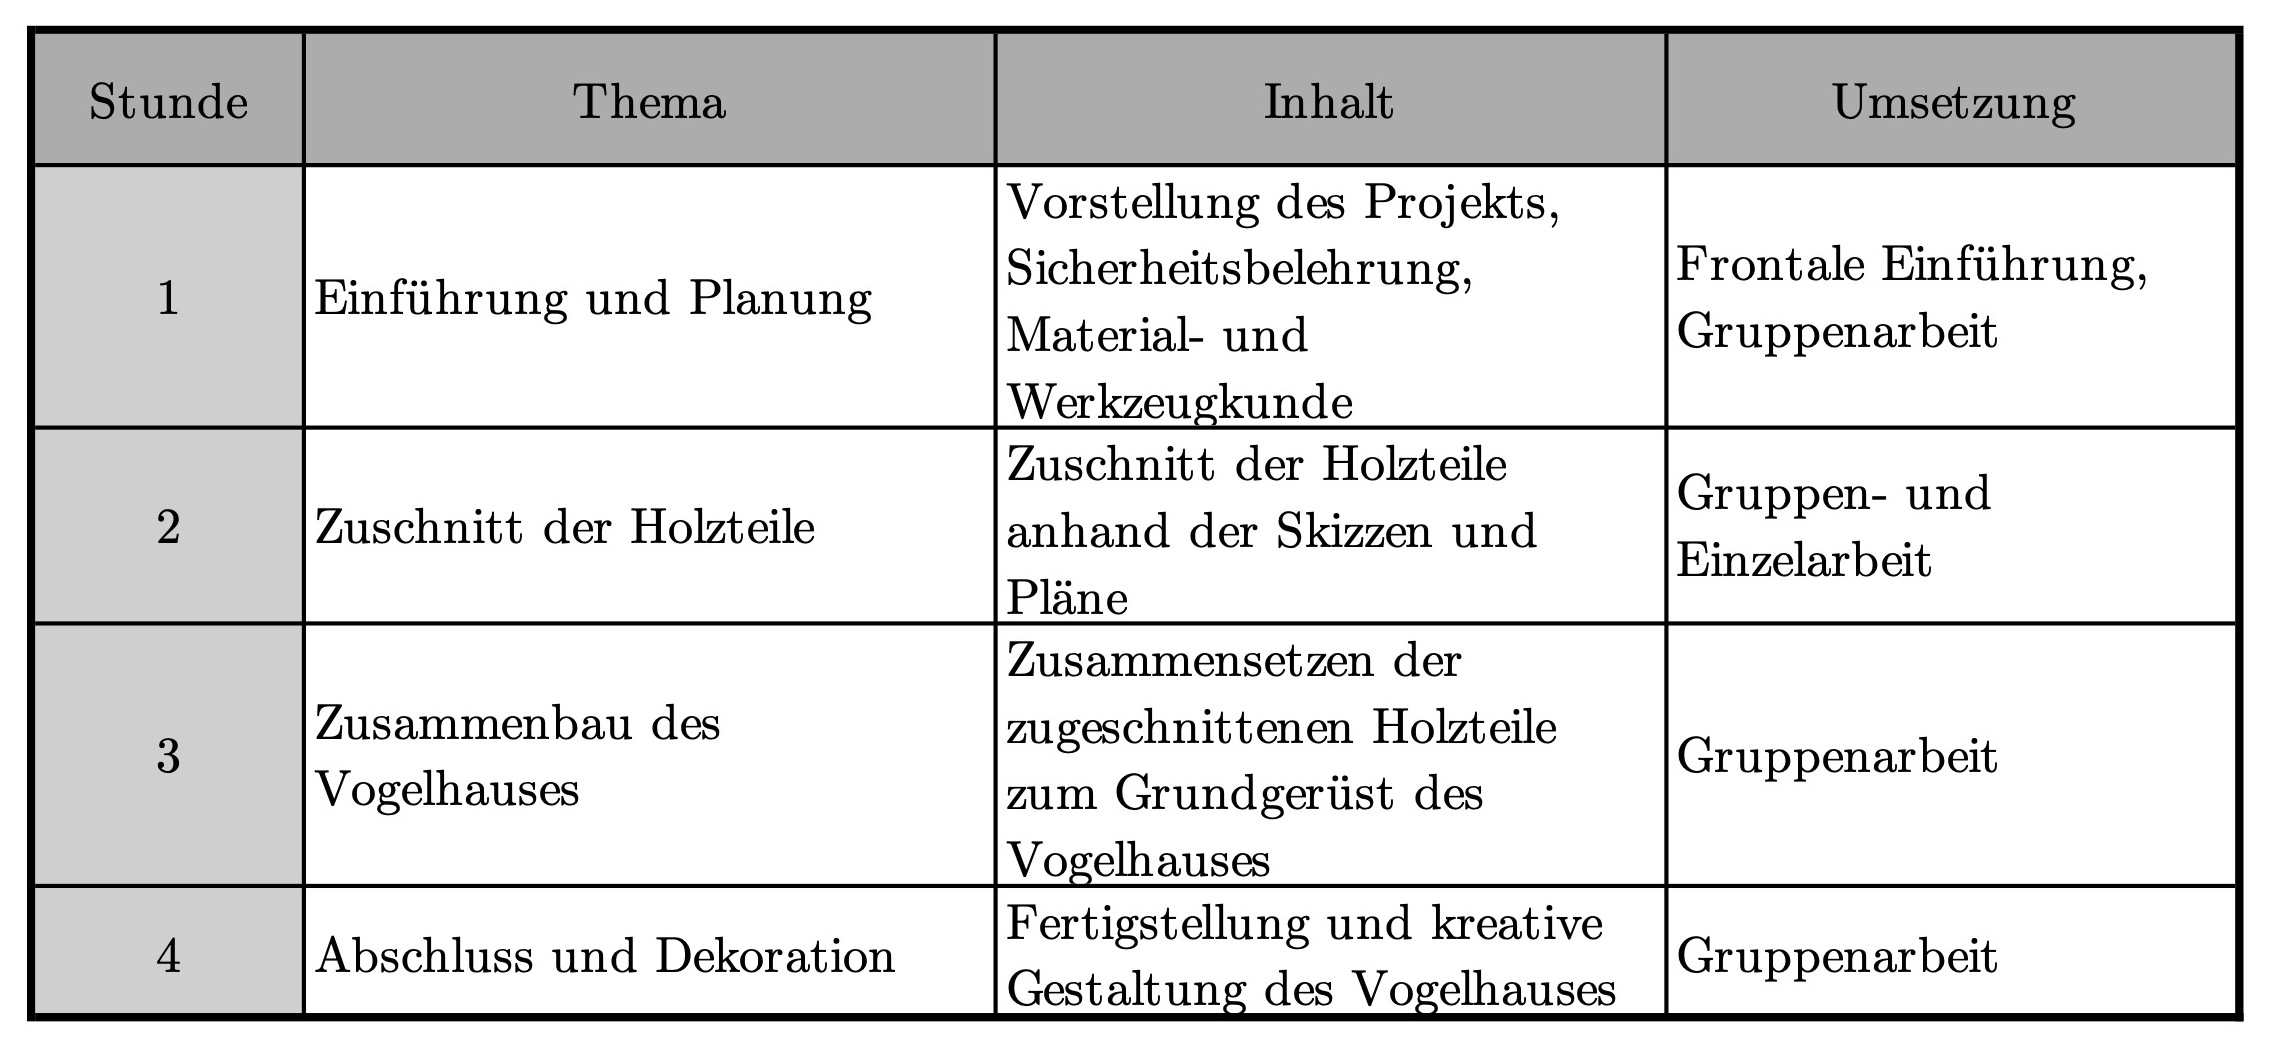
\includegraphics[height=6cm, angle=0, keepaspectratio]{static/Unterrichtsverlauf_Tabelle.jpg}
    \captionof{table}{Tabellarischer Verlaufsplan der Unterrichtsreihe}
\end{center}

\newpage
\section{Vorstellung der Beispielstunden}
Im Folgenden werden die ersten beiden Unterrichtsstunden der geplanten Unterrichtsreihe exemplarisch vorgestellt, inklusive der überlegten didaktischen Handlungen, der Lernziele, geplanten Arbeitsmaterialien und dem Unterrichtsverlauf.


\subsection{Einführungsstunde}
Wie im vorherigen Kapitel erwähnt dient die erste Unterrichtsstunde der Reihe zur Einführung in das Thema, zum Verstehen der Grundlagen bezogen auf Baupläne und Materialien und zur Einführung in Sicherheitsregeln, die im Laufe der Unterrichtsreihe befolgt werden sollen. Der tabellarische Verlaufsplan kann in Anhang A eingesehen werden. Die Lernziele der ersten Unterrichtsstunde lauten (formuliert nach den Formulierungshilfen der TU Dresden \autocite[vgl.][]{sachsisches_e-competence_zertifikat_formulierung_2010}): 

Die Schülerinnen und Schüler...
\begin{itemize}
    \item können die Bauteile eines Vogelhauses benennen und verstehen deren Zusammenhang.
    \item können einen personalisierten Bauplan für ein Vogelhaus erstellen, indem sie ihre bisherigen Erfahrungen kreativ zum Ausdruck bringen.
    \item benennen und begründen ihre Überlegungen sachgerecht.
\end{itemize}

Zu den generellen Unterrichtsvorkehrungen für die Kinder mit Förderbedarf zählen, dass beide Schüler nahe am Lehrer sitzen, ihre Gruppenzuteilung berücksichtigt wird, bzw. generell die Raumbedingungen auf sie angepasst werden (siehe Kapitel 2). Dies wird in der nachfolgenden Beschreibung der Unterrichtsphasen weiter ausgeführt.

Der Unterricht startet mit einer zehnminütigen Einstiegsphase, deren Inhalt die Einführung in da Projekt anhand eines Beispiels ist, um eine Zielvorstellung für die Unterrichtsreihe hervorzurufen. Dies geschieht im Plenum und mithilfe eines beispielhaften, fertigen Vogelhauses, das vorab vorbereitet wurde, sowie einer Abbildung dessen (und dessen Bauplans), wie es in Anhang C und D zu sehen ist. Ziel ist es in dieser Phase das Interesse der Schülerinnen und Schüler zu wecken, was zu einer Motivationssteigerung führen soll. Hier ist wichtig, dass die visuelle Vorstellung für beide Kinder mit Förderbedarf von Bedeutung ist (vgl. Kapitel 2), um ihren Förderbedarfen gerecht zu werden, sowie auch als multisensorische Unterrichtskomponente für die verschiedenen Lernstile der anderen Schülerinnen und Schüler 

Darauf folgt eine zehnminütige Phase zur Material- und Werkzeugkunde, inklusive einer Sicherheitsbelehrung, die auch im Plenum stattfindet. Hier werden die Werkzeuge und Materialien, die in der praktischen Phase der Unterrichtsreihe genutzt werden (eine Japansäge, 3mm Sperrholzplatten) visuell sichtbar vorgestellt, sowie deren Nutzung praktisch vorgeführt. Dies soll vertieft werden mit dem von \textit{Die Werkkiste} erstellten YouTube-Videos zur Werkzeugkunde \Autocite{die_werkkiste_werkzeugfuhrerschein_2018}, um einen weiteren visuellen und auditiven Anreiz für alle Schülerinnen und Schüler - auch denen mit Förderbedarf - bereitzustellen. Des Weiteren sollen in der praktischen Vorführung bereits die später vorgestellten Sicherheitsvorkehrungen aufgezeigt werden, um die Schülerinnen und Schüler schon zum Start der Unterrichtsreihe für deren Wichtigkeit zu sensibilisieren. Ziel ist es, die benötigten Kenntnisse über die Materialien zu vermitteln, als auch ein Bewusstsein für die Sicherheitsvorkehrungen zu schaffen. 

Die darauffolgende, fünfzehnminütige Unterrichtsphase umfasst die Einführung in das Arbeiten mit Bauplänen und die Stundenaufgabe. Dies geschieht erneut im Plenum in einer multisensorischen Form, um möglichst viele Lernstile und die Schüler mit Förderbedarf anzusprechen, indem speziell das beispielhaft vorbereitete Baustück, als auch die Folie zur Vorstellung des Bauplans (Anhang C und D) frontal vorgestellt und deren Aufbau, bzw. Zusammenhang erklärt werden, sowie die Arbeitsschritte zum Bau eines Vogelhauses dargestellt werden. Ziel dieser Aufgabenerklärung ist es ein Verständnis für den Zusammenhang zwischen Bauplan und Endprodukt hervorzurufen, um so die Bearbeitung der Aufgabenstellung zu gewährleisten, und die Schüler mit Förderbedarf bestmöglich zu inkludieren. Dafür sollten hier die Aufgabenblätter für die erste Unterrichtsstunde (Anhang E) ebenfalls frontal erklärt und vorgeführt werden. Die Aufgabenblätter sind sehr einfach gestaltet, mit wenig Text in großer Schriftart, um das Lesen für die Schülerin Jana zu erleichtern. Außerdem gibt es zusätzliche schrittweise Ausführungsrichtlinien zur Aufgabenstellung, was ebenfalls zur Unterstützung von Jana dient (vgl. Kapitel 2). Für Jens ergibt sich aus der generellen visuellen Unterstützung ein Vorteil, aber auch alle anderen Schülerinnen und Schüler mit tendenz zum visuellen Lerntypen 

Nachdem die Aufgabenstellung eingeführt wurde, startet die vierte, zwanzigminütige Unterrichtsphase in Form einer Gruppenarbeit. Hier sollen die Schülerinnen und Schüler das Grundaussehen ihres Vogelhauses planen und die jeweiligen Seiten innerhalb der Gruppe verteilen, was einen zwischenmenschlichen Austausch und die Zusammenarbeit anregen soll. Hierzu kriegt jede Gruppe eine Sammlung von Aufgabenblättern, sowie einen ersten Ausdruck der Sicherheitsbelehrung (Anhänge E-F). Die Schüler können so besonders das Verständnis für den Zusammenhang von Bauplan, der Bauteile und dem späteren Aussehen des Vogelhauses vertiefen, sowie eine erste begründete Überlegung zur personalisierten, kreativen Idee für das Endprodukt formulieren und diskutieren. Ziel dieser Phase ist es, die Kommunikationskompetenz, sowie die organisatorischen-, sozialen- und motorischen Fähigkeiten zu fördern 

In der letzten, fünfminütigen Unterrichtsphase soll eine Kurzvorstellung der Gruppenpläne gemacht und eine kritische Reflexion der des Unterrichts angeregt werden, um sowohl die Fähigkeit zur Reflexion als auch die Kommunikationskompetenz zu fördern. Dies dient außerdem als Feedback für die Lehrkraft, um gegebenenfalls Änderungen am restlichen Verlauf der Unterrichtsreihe vorzunehmen. Insgesamt bereitet die erste Unterrichtsstunde die Schülerinnen und Schüler auf die Unterrichtsreihe vor und führt in die wichtigsten Themenbereiche zur Vervollständigung dieser ein, während die vorab formulierten Lernziele erreicht und Maßnahmen zur Inklusion eingesetzt werden.

\subsection{Zuschnitt der Holzteile}
Die zweite Unterrichtsstunde der Reihe fokussiert sich auf den praktischen Zuschnitt der Holzteile für das Vogelhaus, wobei die Schülerinnen und Schüler ihre motorischen Fähigkeiten sowie ihr Verständnis für Baupläne vertiefen sollen. Der detaillierte tabellarische Verlaufsplan kann in Anhang B eingesehen werden. Die Lernziele der zweiten Unterrichtsstunde lauten (formuliert nach den Formulierungshilfen der TU Dresden \autocite[vgl.][]{sachsisches_e-competence_zertifikat_formulierung_2010}): 

Die Schülerinnen und Schüler...
\begin{itemize}
    \item können einem Bauplan die Fertigungsschritte entnehmen und einen für sie effizienten Fertigungsweg abschätzen.
    \item können Sicherheitsvorkehrungen beachten und Regeln befolgen.
    \item können die geplante handlungsorientierte, handwerkliche Werkzeugarbeit anwenden.
\end{itemize}

Zu den besonderen Unterrichtsvorkehrungen zählen auch in dieser Stunde Maßnahmen zur Differenzierung für die Kinder mit Förderbedarf. So soll Jens - wie in der Einführungsstunde - durch zusätzliche visuelle Zuschnitthilfen, die von der Lehrkraft bereitgestellt werden, unterstützt werden. Bei Jana hingegen wird die Aufgabe durch eine vereinfachte Darstellung der Baupläne und klare, schrittweise Anweisungen strukturiert (siehe Anhang E), um ihren Förderbedarfen gerecht zu werden. Beide Schüler sitzen erneut nahe an der Lehrkraft, um bei Bedarf schnell Unterstützung zu erhalten, und sind den selben, spezifisch ausgewählten Gruppen zugeteilt.

Die zweite Unterrichtsstunde beginnt mit einer zehnminütigen Wiederholungs- und Vorbereitungsphase. Diese dient dazu, den Bauplan und die Sicherheitsbelehrung aus der ersten Stunde zu wiederholen, und die Bedeutung der Sicherheitsregeln zu festigen. Im Plenum wird nochmals auf die relevanten Sicherheitsregeln eingegangen, wobei das Aufgabenblatt 1 und die Sicherheitsbelehrung zur visuellen Unterstützung dienen (siehe Anhänge E und F). Die Sicherheitsvorkehrungen sollen in dieser Phase besonders fokussiert werden, und sind ähnlich wie die Aufgabenstellung in anbetracht der Förderschwerpunkte gestaltet worden (große Überschriften, wenig Text auf dem Blatt, farblich hervorgehobene, kurze Begriffe für jede Sicherheitsregel) (siehe Kapitel 2). Deshalb ist in Form dieser die Hervorhebung von Janas Förderbedarf zu sehen, bei Jens sollte hier besonders auf den Sitzplatz und die Raumbedingungen geachtet werden \autocite[vgl.][]{prof_dr_thomas_kaul_forderschwerpunkt_2016}. Ziel dieser Unterrichtsphase ist es, das aus der ersten Unterrichtsstunde mitgenommene Wissen aufzufrischen, neben der Verinnerlichung der Sicherheitsbedeutung.

In der darauf folgenden Demonstrationsphase von ebenfalls zehn Minuten wird der Zuschnitt der Holzteile frontal von der Lehrkraft demonstriert. Diese Phase findet im Plenum statt, wobei die Japansäge und die 3mm Sperrholzplatten verwendet werden. Außerdem wird die Sicherheitsausrüstung, bestehend aus Schutzbrille und Handschuhen, vorgestellt und deren richtige Handhabung demonstriert. Hierbei sollen die Kenntnisse über das genutzte Material und Werkzeug vertieft sowie ein Sicherheitsbewusstsein geschaffen werden. Zudem werden Regeln aufgestellt, die während der Arbeitsphase einzuhalten sind, und welche aus der Sicherheitsbelehrung übernommen werden, was zu einer Wiederholung und Sicherung dieser führt. Die multisensorische Präsentation richtet sich besonders an die unterschiedlichen Lerntypen der Schülerinnen und Schüler, inklusive derer mit Förderbedarf, um einen einheitlichen und sicheren Arbeitsprozess zu gewährleisten. Ziel ist es, die Techniken des Holzschneidens kennenzulernen, zu wiederholen und die Kompetenz im Umgang mit den Werkzeugen aufzubauen.

Anschließend folgt eine dreißigminütige Arbeitsphase, in der die Schülerinnen und Schüler selbstständig den Zuschnitt der Holzteile in Gruppenarbeit durchführen. Jede Gruppe arbeitet mit dem bereitgestellten Werkzeug und Material, wobei die zuvor demonstrierten Sicherheitsmaßnahmen strikt beachtet werden müssen. Hier liegt weniger der Fokus auf den selbsterstellten Bauplänen und der kreativen Gestaltung der eigenen Seite, sondern der Zusammenarbeit beim Bau der Basiskonstruktion. Während dieser Phase begleitet die Lehrkraft die Arbeit der Gruppen eng und gibt Hilfestellung wenn nötig, insbesondere bei den Schülern mit Förderbedarf. Auch kontrolliert sie die Einhaltung der Sicherheitsregeln. Ziel dieser Unterrichtsphase ist es, handwerkliche Fähigkeiten zu entwickeln, bzw. zu fördern, und praxisorientiert zu lernen. Die handlungsorientierte Lernform ist besonders für die Schüler mit Förderbedarf von relevanz, genauso wie die schrittweisen, visuellen und strukturierten schriftlichen Handlungs- und Sicherheitsanweisungen (siehe Kapitel 2).

Die Unterrichtsstunde endet mit einer zehnminütigen Reflexions- und Aufräumphase. Im Plenum wird die Arbeit reflektiert, wobei die Schülerinnen und Schüler über die durchgeführten Arbeitsschritte sprechen und diese kritisch hinterfragen sollen. Dabei wird auf die individuellen Arbeitsprozesse und die Gruppendynamik eingegangen. Abschließend wird die Arbeitsfläche gemeinsam aufgeräumt, was wiederum die Einhaltung der letzten Sicherheitsanweisung beinhaltet. Ziel dieser Phase ist es, die Kommunikationskompetenz sowie die organisatorischen, sozialen und motorischen Fähigkeiten der Schülerinnen und Schüler zu fördern. Des Weiteren soll die Arbeitsdisziplin durch das festigen von Ordnung am Arbeitsplatz gestärkt werden. Die Reflexion bietet zudem der Lehrkraft die Möglichkeit, den weiteren Verlauf der Unterrichtsreihe anzupassen und individuelle Unterstützung zu gewähren, falls notwendig.

\subsection{Weiterer Unterrichtsverlauf und Fazit}

Der weitere Verlauf der Unterrichtsreihe - so wie er in Kapitel 3.4.2 vorgestellt wurde - ist flexibel gestaltet, sodass er basierend auf den Erfahrungen und Ergebnissen der ersten Unterrichtsstunden angepasst werden kann. Da jede Klasse und jedes Lernsetting unterschiedliche Anforderungen und Bedürfnisse aufweist, ist es wichtig, den Fortschritt der Schülerinnen und Schüler kontinuierlich zu beobachten und den Unterrichtsverlauf entsprechend zu verändern. Die Struktur der Reihe ist so konzipiert, dass bei Bedarf Anpassungen in Bezug auf Inhalte, Materialien und Methoden unkompliziert vorgenommen werden können, um die geplanten Lernziele zu erreichen und eine optimale Lernumgebung, die sowohl die Inklusion als auch die individuellen Lernfortschritte aller Schülerinnen und Schüler berücksichtigt, zu schaffen.

Die vorliegende Hausarbeit skizziert eine Unterrichtsreihe, die sowohl theoretische als auch praktische Aspekte des Unterrichts kombiniert, um Schülerinnen und Schülern ein umfassendes Verständnis für den Bau eines Vogelhauses zu vermitteln. Die Unterrichtsreihe berücksichtigt dabei nicht nur die allgemeinen Lernziele, sondern auch die speziellen Bedürfnisse von Schülern mit Förderbedarf, indem sie differenzierte Methoden und Materialien einsetzt, die auf die Anforderungen des Kernlehrplans angepasst sind.

Die geplante Reihe verfolgt das Ziel, sowohl die handwerklichen Fähigkeiten als auch die sozialen Kompetenzen der Schülerinnen und Schüler zu fördern. Gleichzeitig wird ein Bewusstsein für Sicherheitsvorkehrungen und die Bedeutung von sorgfältiger Planung geschaffen. Insgesamt trägt die Unterrichtsreihe dazu bei, den Schülern wichtige Kompetenzen zu vermitteln, die über das reine Fachwissen hinausgehen und sie in ihrer persönlichen Entwicklung unterstützen. Sie ist zwar theoretisch geplant, könnte aber im weiteren praktischen Diskurs von einer Lehrkraft umgesetzt und erprobt werden, was weitere interessante wissenschaftliche Konversationen ermöglicht.


% print bibliography with heading in table of contents
\newpage
\printbibliography[heading=bibintoc]
\pagestyle{empty}

% Starte Anhang
\newpage
\begin{appendices}

    % Sektionen
    \section{Tabellarischer Verlaufsplan zur ersten Unterrichtsstunde}
    \begin{center}
        \includegraphics[height=14cm, angle=90, keepaspectratio]{static/Unterrichtsstunde_1_Tabelle.pdf}
        \captionof{table}{Tabellarischer Verlaufsplan zur ersten Unterrichtsstunde}
    \end{center}
    
    \section{Tabellarischer Verlaufsplan zur zweiten Unterrichtsstunde}
    \begin{center}
        \includegraphics[height=14cm, angle=90, keepaspectratio]{static/Unterrichtsstunde_2_Tabelle.pdf}
        \captionof{table}{Tabellarischer Verlaufsplan zur zweiten Unterrichtsstunde}
    \end{center}

    \section{Abbildung eines Beispielhaften Vogelhauses}
    \begin{center}
        \vspace{1cm}
        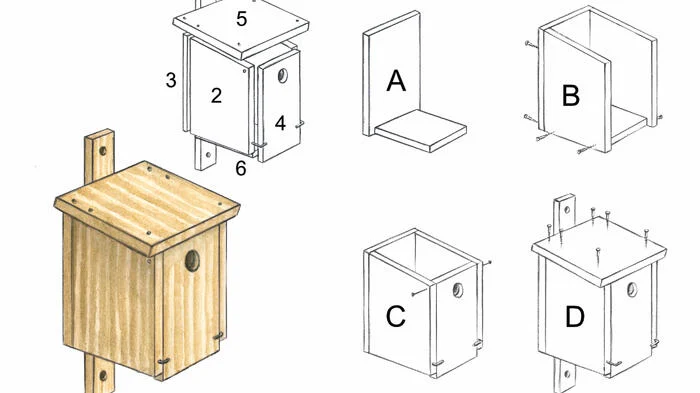
\includegraphics[width=10cm, keepaspectratio]{static/Beispiel-Vogelhaus.png}
        \captionof{figure}{Beispielhaftes Vogelhaus \parencite{noauthor_vogelhaus_nodate-1}}
    \end{center}

    \section{Folie zur Vorstellung des Bauplans}
    \begin{center}
        \vspace{1cm}
        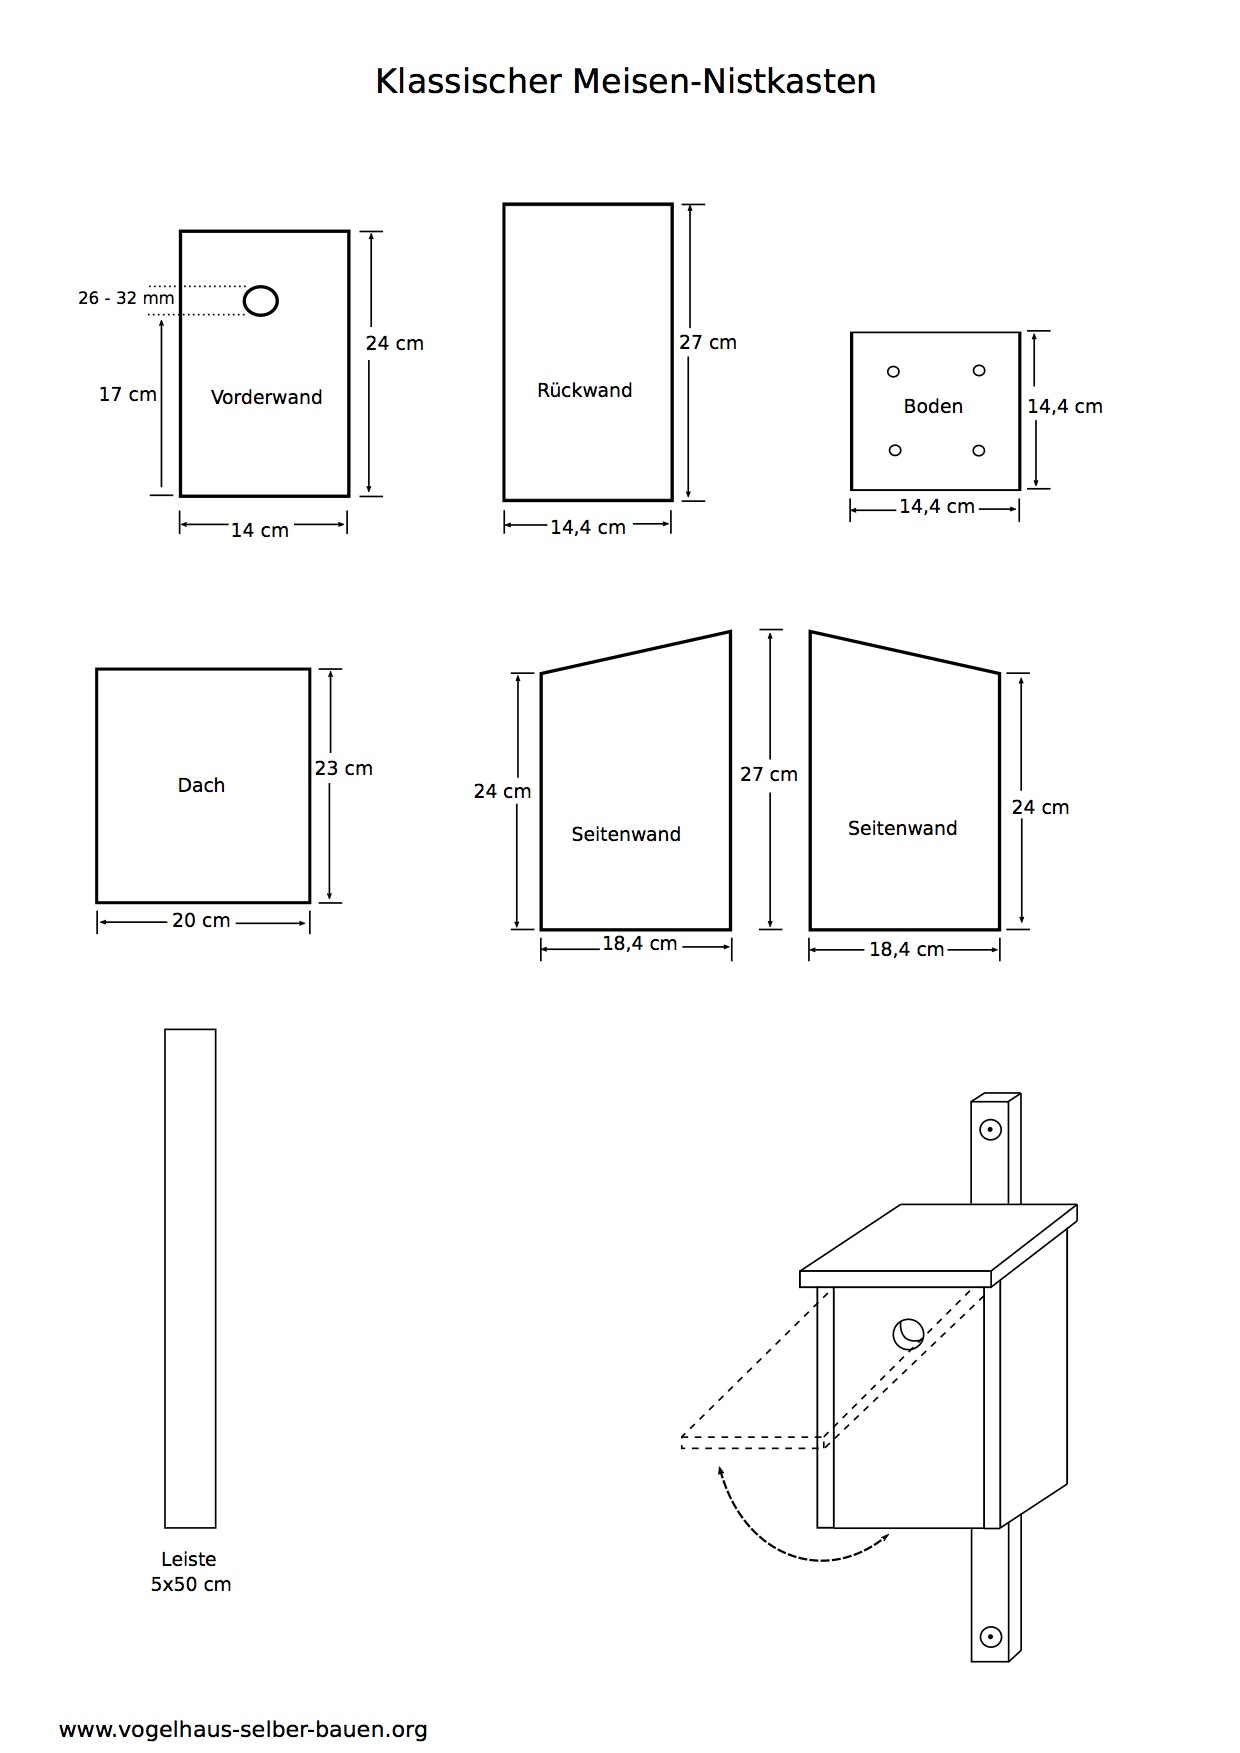
\includegraphics[width=10cm, keepaspectratio]{static/Bauplan-Vogelhaus.jpg}
        \captionof{figure}{Beispielhafter Bauplan \parencite{noauthor_vogelhaus_nodate}}
    \end{center}

    \section{Aufgabenblätter zur ersten Unterrichtsstunde}
    \begin{center}
        \vspace{0cm}
        \includegraphics[height=21cm, keepaspectratio]{static/Aufgabenblatt1.pdf}
        \captionof{figure}{Aufgabenblatt 1 - Aufgabenstellung}
        \vspace{2cm}
        \includegraphics[height=21cm, keepaspectratio]{static/Aufgabenblatt2.pdf}
        \captionof{figure}{Aufgabenblatt 2 - Bauplan der Rückwand}
        \vspace{2cm}
        \includegraphics[height=21cm, keepaspectratio]{static/Aufgabenblatt3.pdf}
        \captionof{figure}{Aufgabenblatt 3 - Bauplan der Vorderwand}
        \vspace{2cm}
        \includegraphics[height=21cm, keepaspectratio]{static/Aufgabenblatt4.pdf}
        \captionof{figure}{Aufgabenblatt 4 - Bauplan der Seitenwand 1}
        \vspace{2cm}
        \includegraphics[height=21cm, keepaspectratio]{static/Aufgabenblatt5.pdf}
        \captionof{figure}{Aufgabenblatt 5 - Bauplan der Seitenwand 2}
    \end{center}

    \section{Sicherheitsbelehrung}
    \begin{center}
        \vspace{2cm}
        \includegraphics[height=21cm, keepaspectratio]{static/Sicherheitsbelehrung.pdf}
        \captionof{figure}{Sicherheitsbelehrung}
    \end{center}

    \section{Eidesstattliche Versicherung}
    \begin{center}
        \vspace{2cm}
        \includegraphics[height=21cm, keepaspectratio]{static/Eidesstattliche-Versicherung.pdf}
        \captionof{figure}{Eidesstattliche Versicherung}
    \end{center}

\end{appendices}

\end{document}